% Тип документа
\documentclass[a4paper,14pt]{extarticle}

% Шрифты, кодировки, символьные таблицы, переносы
\usepackage[utf8]{inputenc}
\usepackage[russian]{babel}
% Это пакет -- хитрый пакет, он нужен но не нужен
\usepackage[mode=buildnew]{standalone}

\usepackage
    {
        % Дополнения Американского математического общества (AMS)
        amssymb,
        amsfonts,
        amsmath,
        amsthm,
        % Пакет для физических текстов
        physics,
        % misccorr,
        % 
        % Графики и рисунки
        float,
        geometry,
        graphicx,
        % 
        % Интегралы и прочие обозначения
        ulem,
        esint,
        esdiff,
        % 
        % Колонтитулы
        fancyhdr,
    } 
    
\usepackage{mathtools}
\mathtoolsset{showonlyrefs=true} 

\usepackage{xcolor}
\usepackage{hyperref}
 % Цвета для гиперссылок
\definecolor{linkcolor}{HTML}{000000} % цвет ссылок
\definecolor{urlcolor}{HTML}{799B03} % цвет гиперссылок
 
\hypersetup{linkcolor=linkcolor,urlcolor=urlcolor, colorlinks=true}
\hypersetup{pageanchor=false}
% Увеличенный межстрочный интервал, французские пробелы
\linespread{1.3} 
\frenchspacing 

\newcommand{\mean}[1]{\langle#1\rangle}
\newcommand*{\const}{\ct{const}}
\renewcommand{\phi}{\varphi}
\renewcommand{\hat}{\widehat}
\usepackage{array}

\geometry       
    {
        left            =   2cm,
        right           =   2cm,
        top             =   2.5cm,
        bottom          =   2.5cm,
        bindingoffset   =   0cm
    }

%%%%%%%%%%%%%%%%%%%%%%%%%%%%%%%%%%%%%%%%%%%%%%%%%%%%%%%%%%%%%%%%%%%%%%%%%%%%%%%
    %применим колонтитул к стилю страницы
\pagestyle{fancy} 
    %очистим "шапку" страницы
% \fancyhead{} 
    %слева сверху на четных и справа на нечетных
\fancyhead[R]{\small Понур К.А.}%\labauthors 
    %справа сверху на четных и слева на нечетных
% \fancyhead[L]{Отчёт по лабораторной работе №\labnumber}
\fancyhead[L]{Кафедра общей физики ННГУ им. М.Ю. Лобачевского} 
    %очистим "подвал" страницы
% \fancyfoot{} 
    % номер страницы в нижнем колинтуле в центре
\fancyfoot[C]{} 

%%%%%%%%%%%%%%%%%%%%%%%%%%%%%%%%%%%%%%%%%%%%%%%%%%%%%%%%%%%%%%%%%%%%%%%%%%%%%%%

\renewcommand{\contentsname}{Оглавление}
\usepackage{tocloft}
\usepackage{secdot}
\sectiondot{subsection}


\begin{document}
\section{Линейная частотная модуляция}%
\label{sec:lineinaia_chastotnaia_moduliatsiia}
\begin{figure}[h!]
    \centering
    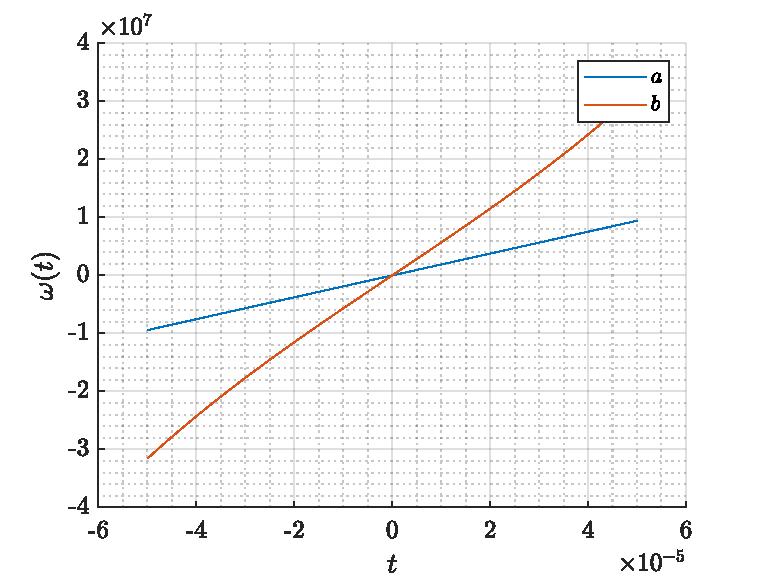
\includegraphics[scale=1]{fig/omega}
    \label{fig:omega}
    \caption{Различные частотные модуляции: (a) линейная частотная модуляция;
    (b) нелинейная частотная модуляция.}
\end{figure}

\begin{figure}[h!]
    \centering
    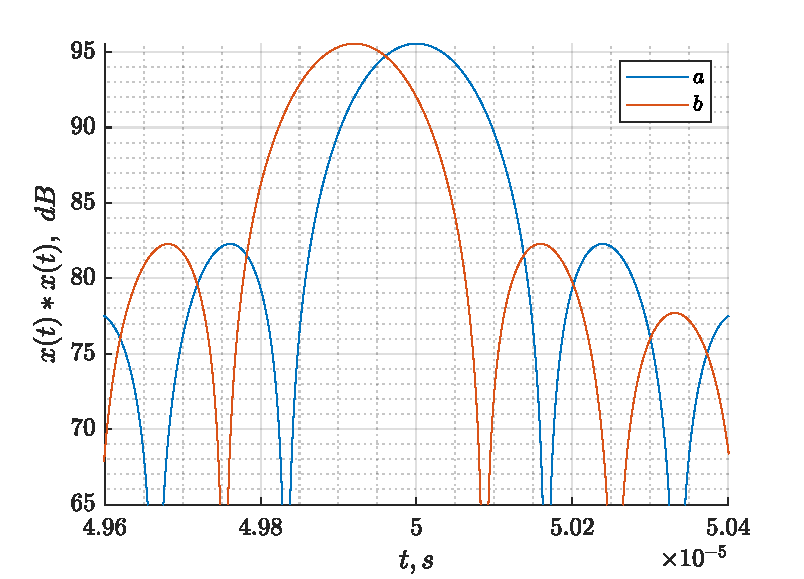
\includegraphics[scale=1]{fig/linear_conv}
    \caption{Свертка детерменированного сигнала $x(t)$ (ЛЧМ) с самим собой.
    (a) без учета допплеровского смещения;
    (b) с учетом допплеровского смещения.}
    \label{fig:linear_conv}
\end{figure}

\begin{figure}[h!]
    \centering
    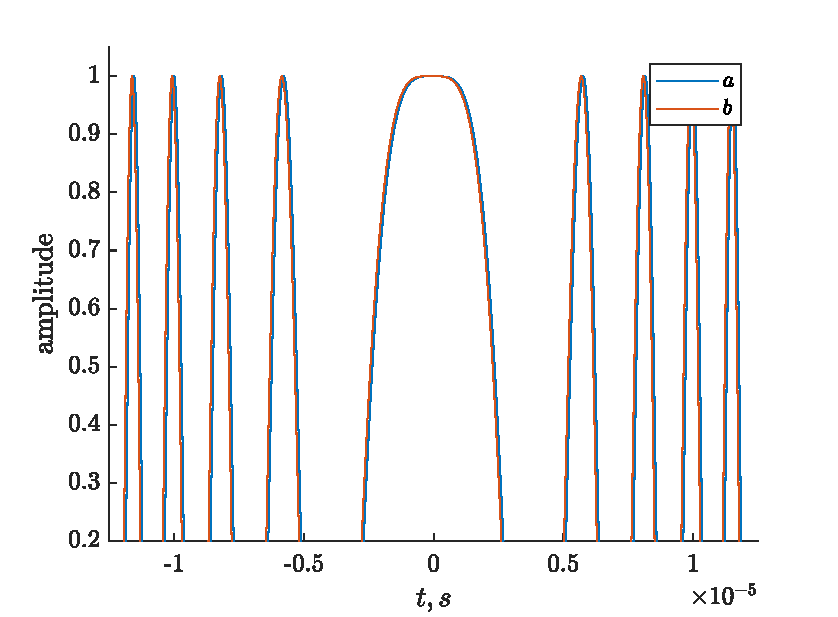
\includegraphics[scale=1]{fig/signal}
    \caption{Детерменированный сигнал $x(t)$ (a) ЛЧМ; (b) НЧМ.}
    \label{fig:signal}
\end{figure}

Рассмотрим сначала линейную зависимость 
\begin{equation}
    \label{eq:linear_omega}
    \omega(t) = 2\pi \Delta f = \frac{t}{\tau},
\end{equation}
где $\Delta f= 3 \text{ МГц}$ -- ширина полосы сигнала,
$\tau=100 \text{ мкс}$ -- длительность сигнала (см. рис.
\ref{fig:omega}a). 

Целью будет являться выделение сигнала вида $x(t) = \exp{ i \omega(t) t}$ (см.
рис. \ref{fig:signal}) из статического шума. 
На практике это означет применение согласованного фильтра, который выполняет
операцию свертки случайного сигнала $\xi(t)$ с детерменированным  $x(t)$
 \begin{equation}
    \label{eq:linear_conv}
    x(t) * \xi(t) = \int\limits_{-\infty}^{\infty}  x(t) \xi^*(t -
    \tau) \dd \tau.
\end{equation}

Но операция нахождение функции свертки процесс ресурсоемкий, поэтому правильнее
воспользовавшись теоремой о свертке
\begin{gather}
    \label{eq:theorem}
    x(t) * \xi(t) = X(\omega) \cdot \Xi^*(\omega),
    \text{ где } \\ 
    X(\omega) = \int\limits_{-\infty}^{\infty} x(t) e^{i \omega t} \dd{t}
    \equiv \mathfrak{F}\qty{x(t)},\\
    \Xi(\omega) = \int\limits_{-\infty}^{\infty} \xi(t) e^{i \omega t} \dd{t}  
    \equiv \mathfrak{F}\qty{\xi^(t)},\\
\end{gather}
перейти в частотную область и считать свертку как обратное Фурье преобразование
спектров сигналов
\begin{equation}
    \label{eq:conv1}
    x(t) * \xi(t) = \frac{1}{2 \pi} \int\limits_{-\infty}^{\infty}   X(\omega)
    \cdot \Xi^*(\omega) e^{-i \omega t} \dd \omega = \mathfrak{F}^{-1}\qty{
    X(\omega) \cdot \Xi^*(\omega)}.
\end{equation}

На рис.\ref{fig:linear_conv}a изображена свертка детерменированного сигнала $x(t)$ с
самим собой, приведенная к логарифмическому масштабу.

\section{Нелинейная частотная модуляция.}%
\label{sec:nelineinaia_chastotnaia_moduliatsiia_}

Нелинейная частотная модуляция спользуется для уменьшения высоты боковых
лепестков у функции свертки $x(t) * x(t)$. В нашем случае НЧМ принимает вид
\begin{equation}
    \label{eq:nonlinear_omega}
    \omega(t) = 2 \pi \Delta f \qty(\frac{t}{\tau} + \cdot
    \sinh(a\frac{t}{\tau})),
\end{equation}
где $a$ -- коэффициеент нелинейности. В предельном случае $a =0$ формула
\eqref{eq:nonlinear_omega} выродится в формулу \eqref{eq:linear_omega}.

Свертка для нелинейного случая изображена на рис. \ref{fig:nonlinear_conv}.

\begin{figure}[h!]
    \centering
    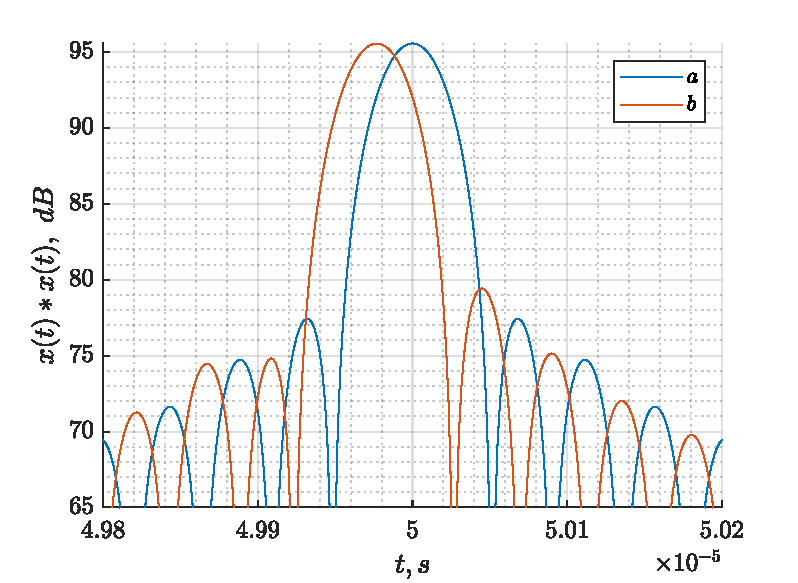
\includegraphics[scale=1]{fig/nonlinear_conv}
    \caption{Свертка детерменированного сигнала $x(t)$ (НЧМ) с самим собой.
    (a) без учета допплеровского смещения;
    (b) с учетом допплеровского смещения.}
    \label{fig:nonlinear_conv}
\end{figure}

Как видно из рис. \ref{fig:nonlinear_conv} боковые лепестки стали меньше, по
сравнению с рис. \ref{fig:linear_conv} примерно на 5 дБ. 

Также, на рис. \ref{fig:nonlinear_conv}b можно заметить что при учете допплеровского
смещения график стал асимметричным: левый лепесток на 4 дБ слабее правого.




\end{document}
